\documentclass[12pt]{article}
\usepackage[utf8]{inputenc}
\usepackage[T1]{fontenc}
\usepackage[spanish]{babel}
\usepackage{indentfirst}
\usepackage{booktabs}
\usepackage{amsmath}
\usepackage{amsfonts}
\usepackage{graphicx}
\usepackage{float}
\usepackage{geometry}
\usepackage{hyperref}

\geometry{letterpaper, margin=2.5cm}
\graphicspath{{figures/}}
\hypersetup{
    colorlinks=true,
    linkcolor=blue,
    urlcolor=blue
}

\title{Informe de Simulación de Eventos Discretos\\Puerto Sobrecargado}
\author{Alberto E. Marichal Fonseca\\Grupo CD 311 \\ \url{https://github.com/ALbertE03/Discrete-event-simulation} }
\date{Mayo de 2026}

\begin{document}

\maketitle

\section{Orden del Problema Asignado}

El problema asignado es \textbf{Puerto Sobrecargado}. Se debe simular el funcionamiento de un puerto de supertanqueros con 3 muelles y un remolcador, con el objetivo de estimar los tiempos promedio de espera y analizar el comportamiento del sistema bajo las reglas de operación indicadas.

En el puerto llegan tanqueros de tres tamaños: pequeños, medianos y grandes. Todos necesitan asistencia del remolcador para entrar al muelle y para abandonar el puerto luego de terminar la carga. Los muelles son recursos limitados y el remolcador es un recurso único, por lo que la congestión puede aparecer tanto antes de entrar al muelle como después de finalizar la carga.

\begin{table}[H]
\centering
\caption{Parámetros de los tanqueros}
\begin{tabular}{lccc}
\toprule
\textbf{Tamaño} & \textbf{Pequeño} & \textbf{Mediano} & \textbf{Grande} \\
\midrule
Probabilidad de arribo & 0.25 & 0.25 & 0.50 \\
Tiempo de carga & $\mathcal{N}(9, 1)$ & $\mathcal{N}(12, 2)$ & $\mathcal{N}(18, 3)$ \\
\bottomrule
\end{tabular}
\end{table}

\section{Principales Ideas Seguidas para la Solución}

La solución se desarrolló como una simulación de eventos discretos. La idea central fue representar cada cambio importante del sistema como un evento futuro y procesar esos eventos en orden cronológico.

\begin{itemize}
    \item Representar los arribos, remolques, cargas y salidas como eventos discretos.
    \item Mantener una lista de eventos futuros usando una cola de prioridad.
    \item Usar una cola FIFO para los barcos que esperan entrar desde el puerto.
    \item Usar una cola FIFO para los barcos que terminaron la carga y esperan salir desde los muelles.
    \item Modelar los 3 muelles mediante un contador de muelles disponibles.
    \item Modelar el remolcador como un recurso único que puede estar en el puerto, en la zona de muelles o viajando.
    \item Reservar un muelle cuando un barco inicia el remolque de entrada para evitar asignaciones duplicadas.
    \item Ejecutar 50 réplicas independientes, cada una con 100000 barcos, para estimar promedios e intervalos de confianza.
\end{itemize}

\section{Modelo de Simulación de Eventos Discretos}

\subsection{Entidades del Modelo}

\begin{itemize}
    \item \texttt{Ship}: representa cada tanquero. Guarda el tipo de barco, hora de llegada, duración de carga, inicio de remolque, inicio y fin de carga, inicio de salida y hora de abandono del sistema.
    \item \texttt{Event}: representa un evento futuro. Tiene tiempo de ocurrencia, tipo de evento y, cuando corresponde, el identificador del barco.
    \item \texttt{PortSimulation}: controla el reloj de simulación, la lista de eventos, las colas, los recursos disponibles y las métricas finales.
\end{itemize}

\subsection{Eventos Implementados}

\begin{enumerate}
    \item \texttt{arrival}: llega un nuevo tanquero al puerto.
    \item \texttt{inbound\_tow\_complete}: termina el remolque de entrada y comienza la carga.
    \item \texttt{loading\_complete}: termina la carga y el barco pasa a la cola de salida.
    \item \texttt{outbound\_tow\_complete}: termina el remolque de salida, el barco abandona el sistema y se libera el muelle.
    \item \texttt{empty\_arrive\_port}: el remolcador llega vacío al puerto.
    \item \texttt{empty\_arrive\_docks}: el remolcador llega vacío a la zona de muelles.
\end{enumerate}

\subsection{Reglas del Remolcador}

Cuando el remolcador está en el puerto, primero intenta llevar al muelle al primer barco de la cola de entrada, siempre que exista al menos un muelle disponible. Si no puede entrar ningún barco y hay barcos esperando salir, viaja vacío hacia los muelles.

Cuando el remolcador está en los muelles, primero atiende a los barcos que esperan salir. Si no hay barcos esperando salir y hay barcos esperando entrar con algún muelle disponible, viaja vacío hacia el puerto.

\subsection{Generación de Variables Aleatorias}

En el notebook se usó directamente la función \texttt{random.expovariate(L)} con los valores indicados para cada proceso. Esta decisión se mantuvo para el análisis, pues representa la condición de puerto sobrecargado usada en las corridas.

\begin{table}[H]
\centering
\caption{Parámetros usados en la simulación}
\begin{tabular}{lc}
\toprule
\textbf{Proceso} & \textbf{Parámetro usado en \texttt{expovariate(L)}} \\
\midrule
Tiempo entre arribos & $\lambda = 8.0$ \\
Remolque de entrada & $\lambda = 2.0$ \\
Remolque de salida & $\lambda = 1.0$ \\
Viaje vacío del remolcador & $\lambda = 0.25$ \\
\bottomrule
\end{tabular}
\end{table}

Para los tiempos de carga se usaron distribuciones normales según el tipo de barco. Si una normal generaba un valor menor o igual que cero, se rechazaba y se volvía a muestrear.

\subsection{Métricas Calculadas}

Para cada barco completado se calcularon las siguientes métricas:

\begin{itemize}
    \item \textbf{Espera antes del remolque de entrada:} \texttt{inbound\_tow\_start - arrival\_time}.
    \item \textbf{Tiempo hasta comenzar carga:} \texttt{loading\_start - arrival\_time}.
    \item \textbf{Espera en muelle para salir:} \texttt{outbound\_tow\_start - loading\_end}.
    \item \textbf{Tiempo total en el sistema:} \texttt{departure\_time - arrival\_time}.
\end{itemize}

Los intervalos de confianza al 95\% se calcularon mediante:

\[
IC_{95\%} = \bar{x} \pm 1.96 \cdot \frac{s}{\sqrt{n}},
\]

donde $n=50$ réplicas.

\section{Resultados de la Simulación}

La configuración base simulada fue la del problema original: 3 muelles, 1 remolcador, 100000 barcos por réplica y 50 réplicas independientes. Los resultados de la Tabla \ref{tab:resultados-base} fueron obtenidos ejecutando el notebook con la lógica descrita.

\begin{table}[H]
\centering
\caption{Resultados de la configuración base}
\label{tab:resultados-base}
\resizebox{\textwidth}{!}{%
\begin{tabular}{lrrrr}
\toprule
\textbf{Métrica} & \textbf{Media (h)} & \textbf{IC 95\% (h)} & \textbf{Mín. (h)} & \textbf{Máx. (h)} \\
\midrule
Espera antes del remolque de entrada & 260314.31 & $\pm$ 66.05 & 259764.87 & 261018.66 \\
Tiempo hasta comenzar carga & 260314.81 & $\pm$ 66.05 & 259765.37 & 261019.17 \\
Espera en muelle para salir & 0.2403 & $\pm$ 0.0007 & 0.2333 & 0.2456 \\
Tiempo total en el sistema & 260330.31 & $\pm$ 66.06 & 259780.83 & 261034.69 \\
\bottomrule
\end{tabular}
}
\end{table}

El tiempo promedio de espera en muelle para salir fue de $0.2403$ horas, equivalente aproximadamente a $14.42$ minutos. Sin embargo, la espera antes de iniciar el remolque de entrada fue extremadamente alta: $260314.31$ horas en promedio. Esto confirma que la congestión principal aparece antes de que los barcos logren entrar al muelle.

\begin{figure}[H]
\centering
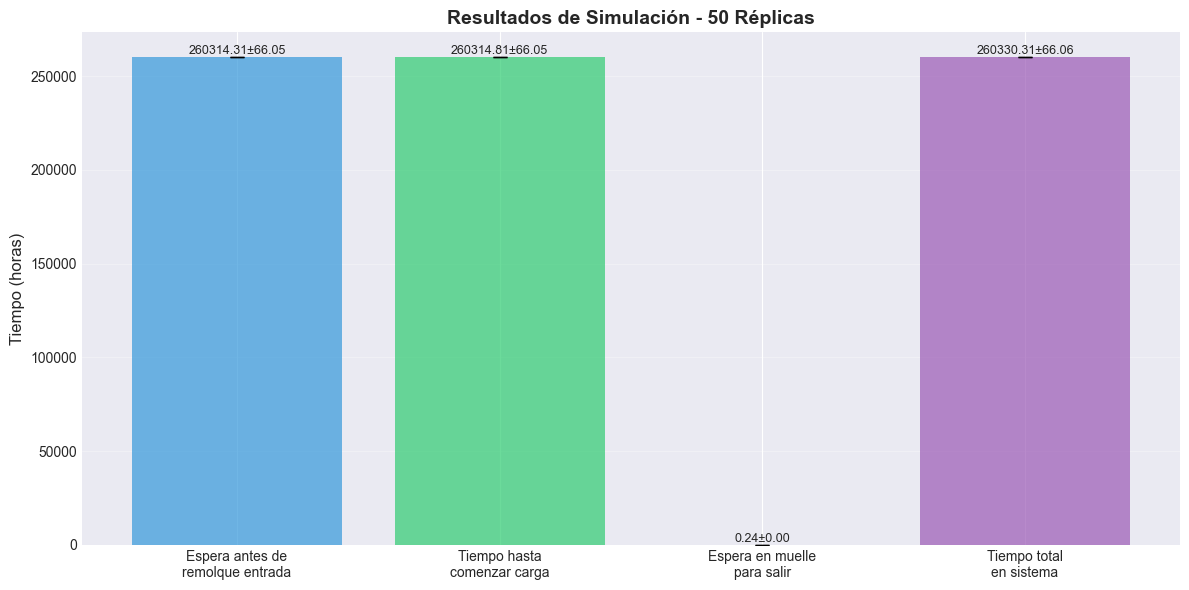
\includegraphics[width=0.95\textwidth]{resultados_metricas.png}
\caption{Promedios e intervalos de confianza de las métricas principales.}
\end{figure}

\begin{figure}[H]
\centering
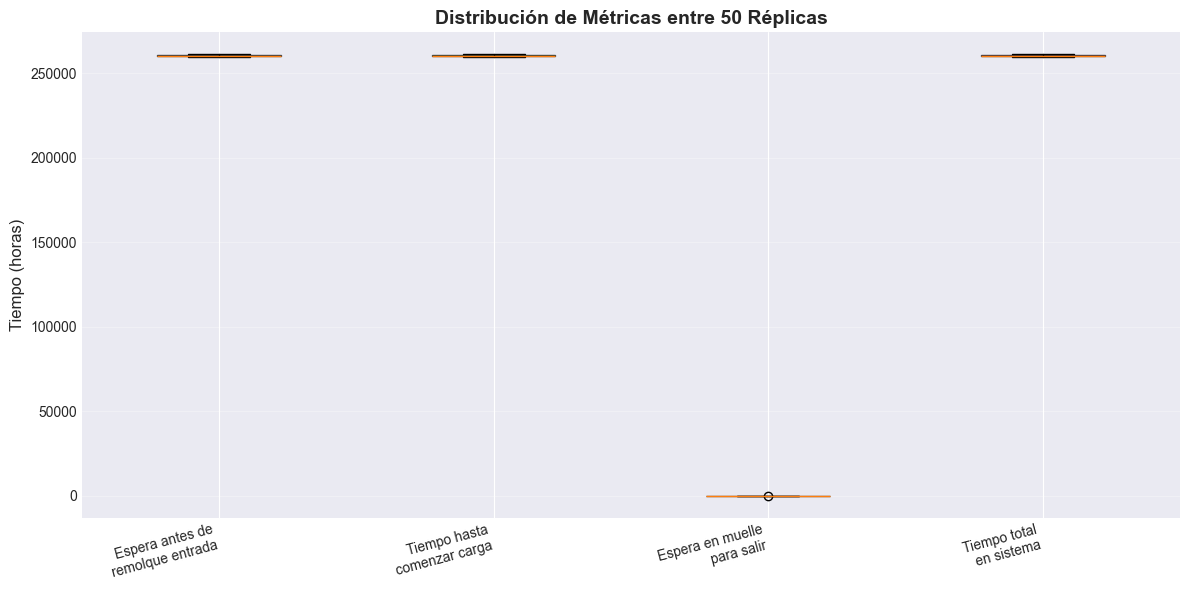
\includegraphics[width=0.95\textwidth]{distribucion_metricas.png}
\caption{Distribución de las métricas entre las 50 réplicas.}
\end{figure}

\begin{figure}[H]
\centering
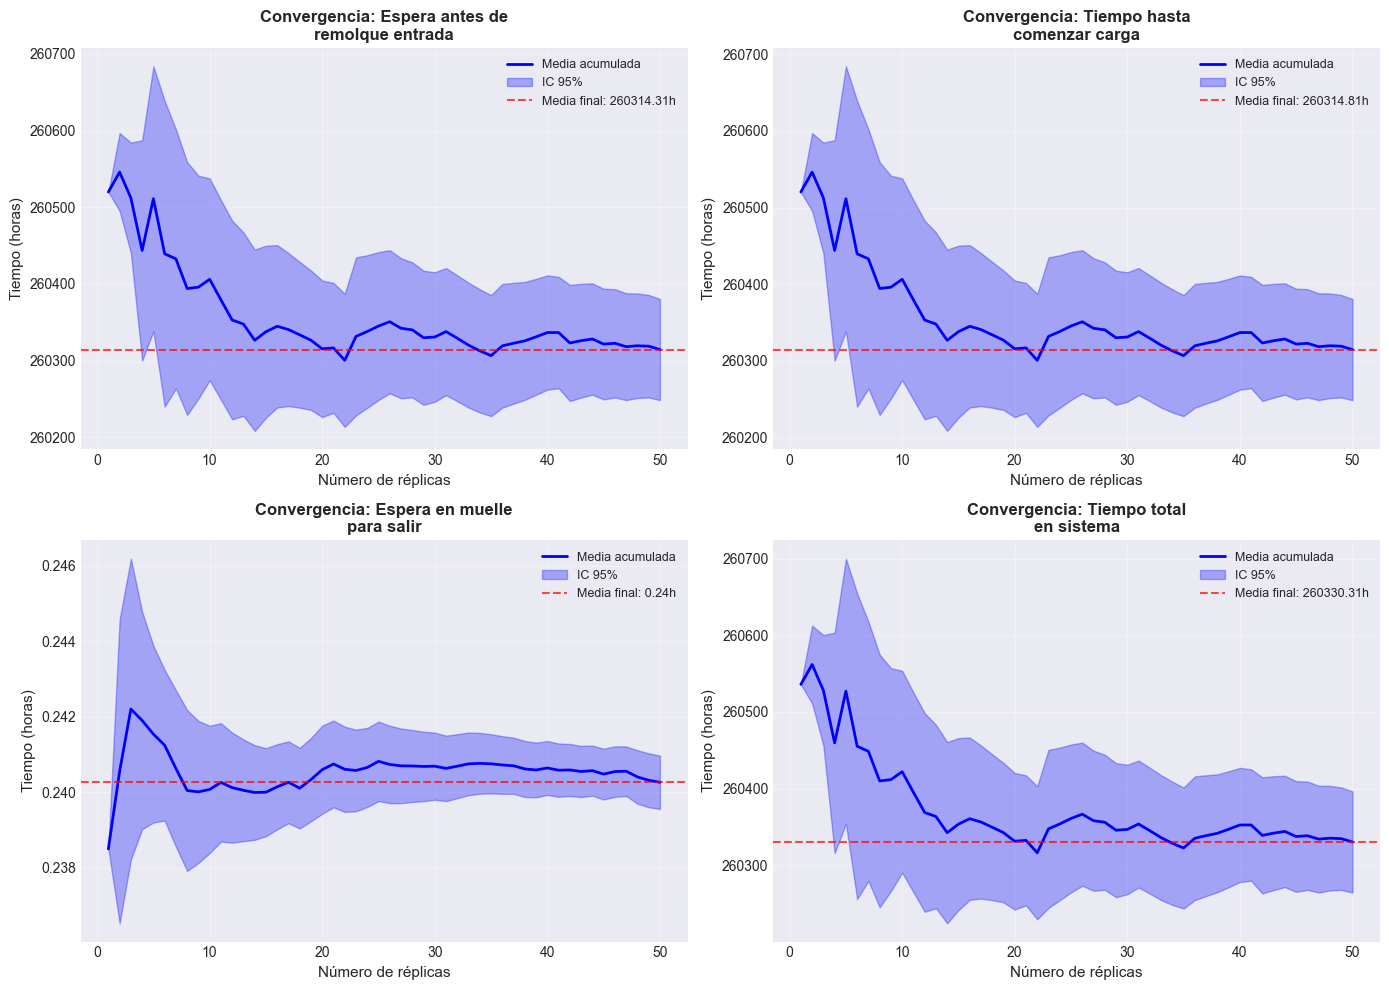
\includegraphics[width=0.95\textwidth]{convergencia_metricas.png}
\caption{Convergencia de las medias acumuladas y sus intervalos de confianza.}
\end{figure}

\begin{figure}[H]
\centering
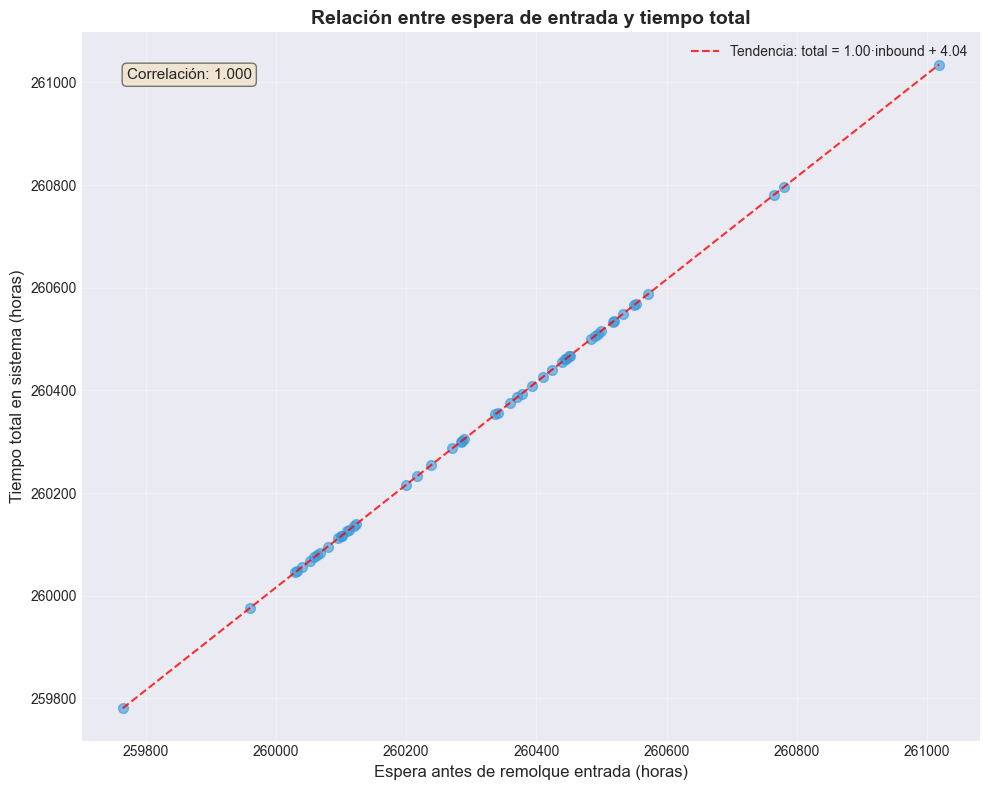
\includegraphics[width=0.82\textwidth]{relacion_espera_total.png}
\caption{Relación entre la espera de entrada y el tiempo total en el sistema.}
\end{figure}

\section{Experimentos con Más Muelles y Remolcadores}

Además de la configuración original, en el notebook se ejecutó un análisis de sensibilidad con diferentes cantidades de muelles y remolcadores. El objetivo de estos experimentos fue observar qué tanto cambia la congestión al aumentar la capacidad del puerto.

Este análisis de sensibilidad usa un esquema de semillas diferente al de la corrida base detallada, por eso la fila \texttt{base\_3\_1} presenta pequeñas variaciones numéricas. La magnitud y la interpretación del comportamiento se mantienen.

\begin{table}[H]
\centering
\caption{Configuraciones evaluadas en el análisis de sensibilidad}
\label{tab:configuraciones}
\resizebox{\textwidth}{!}{%
\begin{tabular}{llcc}
\toprule
\textbf{Identificador} &  & \textbf{Muelles} & \textbf{Remolcadores} \\
\midrule
\texttt{base\_3\_1} & 3 & 1 \\
\texttt{mas\_remolcadores\_3\_2}  & 3 & 2 \\
\texttt{iguales\_3\_3} & 3 & 3 \\
\texttt{mas\_muelles\_4\_1} & 4 & 1 \\
\texttt{mejorado\_4\_2} & 4 & 2 \\
\texttt{extremo\_5\_1} & 5 & 1 \\
\texttt{extremo\_100\_1} & 100 & 1 \\
\texttt{extremo\_100\_50} & 100 & 50 \\
\texttt{extremo\_100\_70} & 100 & 70 \\
\bottomrule
\end{tabular}
}
\end{table}

\begin{table}[H]
\centering
\caption{Resumen de los experimentos de sensibilidad}
\label{tab:sensibilidad}
\resizebox{\textwidth}{!}{%
\begin{tabular}{lccccc}
\toprule
\textbf{Configuración} & \textbf{Muelles} & \textbf{Remolc.} & \textbf{Espera entrada (h)} & \textbf{Tiempo total (h)} & \textbf{Mejora} \\
\midrule
\texttt{base\_3\_1} & 3 & 1 & $260264.61 \pm 82.95$ & $260280.60 \pm 82.96$ & $+0.0\%$ \\
\texttt{mas\_remolcadores\_3\_2} & 3 & 2 & $260259.03 \pm 66.28$ & $260275.02 \pm 66.28$ & $+0.0\%$ \\
\texttt{iguales\_3\_3} & 3 & 3 & $260201.43 \pm 67.11$ & $260217.41 \pm 67.11$ & $+0.0\%$ \\
\texttt{mas\_muelles\_4\_1} & 4 & 1 & $195564.29 \pm 55.51$ & $195580.44 \pm 55.51$ & $+24.9\%$ \\
\texttt{mejorado\_4\_2} & 4 & 2 & $195540.41 \pm 58.42$ & $195556.55 \pm 58.42$ & $+24.9\%$ \\
\texttt{extremo\_5\_1} & 5 & 1 & $157023.57 \pm 48.94$ & $157039.90 \pm 48.94$ & $+39.7\%$ \\
\texttt{extremo\_100\_1} & 100 & 1 & $68821.57 \pm 58.34$ & $68854.25 \pm 58.34$ & $+73.6\%$ \\
\texttt{extremo\_100\_50} & 100 & 50 & $68797.93 \pm 51.02$ & $68830.61 \pm 51.02$ & $+73.6\%$ \\
\texttt{extremo\_100\_70} & 100 & 70 & $68830.43 \pm 55.53$ & $68863.13 \pm 55.58$ & $+73.6\%$ \\
\bottomrule
\end{tabular}
}
\end{table}

\begin{figure}[H]
\centering
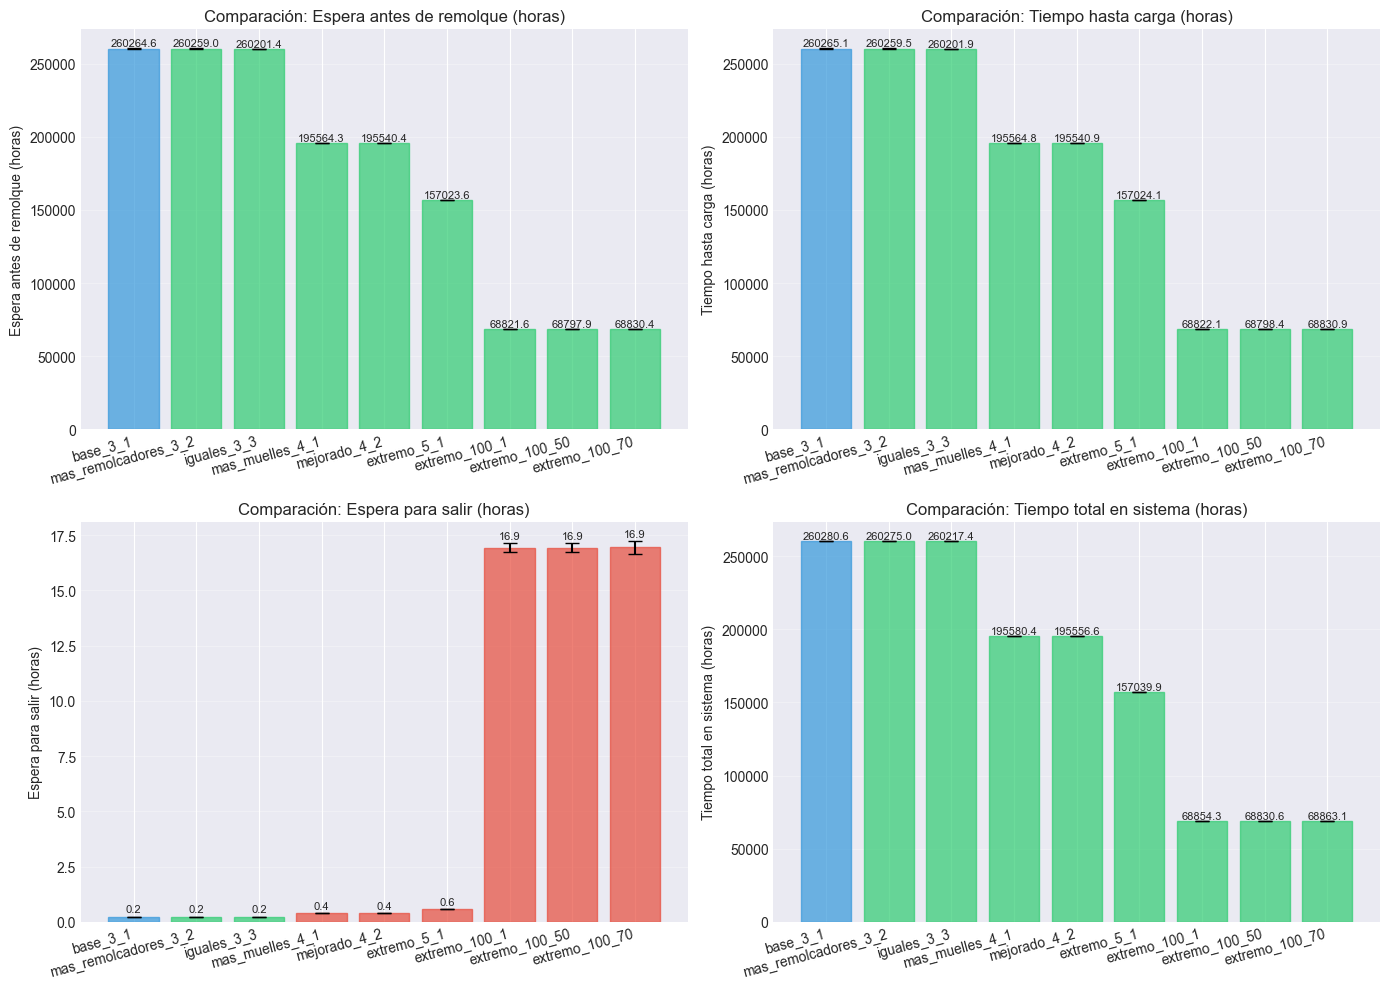
\includegraphics[width=0.95\textwidth]{sensibilidad_comparacion.png}
\caption{Comparación de las métricas principales entre configuraciones.}
\end{figure}

\begin{figure}[H]
\centering
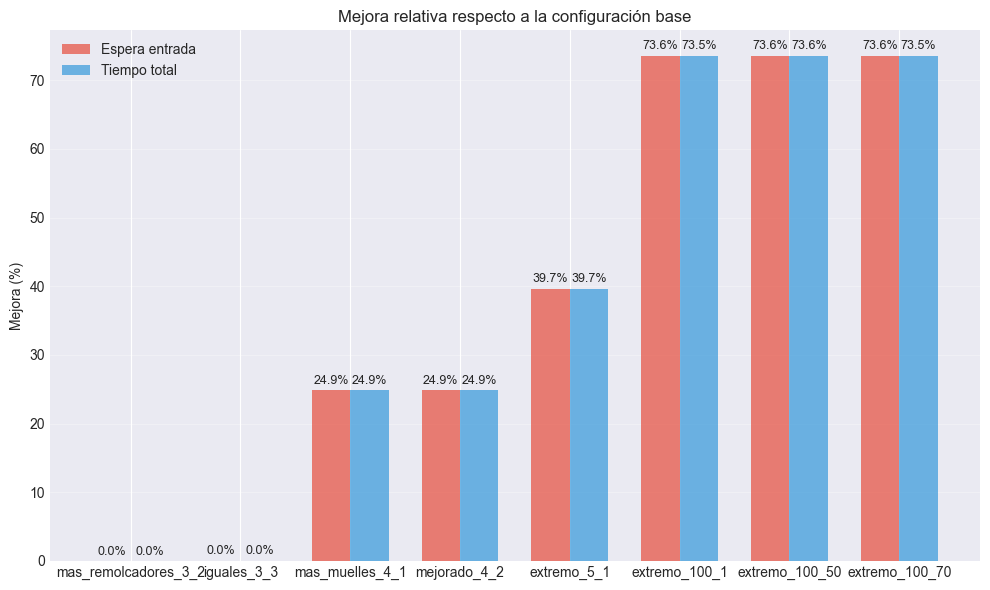
\includegraphics[width=0.90\textwidth]{sensibilidad_mejora_relativa.png}
\caption{Mejora relativa respecto a la configuración base.}
\end{figure}

El análisis ANOVA reportado por el notebook dio diferencias significativas entre configuraciones para la espera de entrada y para el tiempo total en sistema, con $p < 0.05$ en ambos casos. Las comparaciones por pares muestran que aumentar de 3 a 4 muelles, de 4 a 5 muelles y luego hasta 100 muelles reduce de forma significativa la espera de entrada. En cambio, para un mismo número de muelles, aumentar solamente la cantidad de remolcadores no produjo diferencias significativas en las salidas obtenidas.

Los experimentos más interesantes fueron los de aumento de muelles. Pasar de 3 a 4 muelles redujo la espera de entrada en aproximadamente $24.9\%$, mientras que usar 5 muelles alcanzó una mejora cercana al $39.7\%$. Los escenarios extremos con 100 muelles redujeron la espera de entrada en aproximadamente $73.6\%$, aunque el sistema siguió mostrando tiempos de espera elevados por la intensidad de los arribos.

\section{Consideraciones Obtenidas a Partir de las Simulaciones}

Los resultados muestran que el sistema trabaja en una condición de sobrecarga. Con el uso directo de \texttt{expovariate($\lambda$)} y $\lambda=8$ para los arribos, los barcos llegan con mucha frecuencia. La capacidad del puerto queda limitada por los 3 muelles, el remolcador único y los tiempos de carga, especialmente porque la mitad de los tanqueros son grandes y tienen mayor duración de carga.

La métrica de espera antes de entrar al muelle domina el tiempo total en el sistema. La diferencia entre el tiempo hasta comenzar la carga y la espera antes del remolque de entrada es pequeña, lo que indica que, una vez que el barco consigue ser atendido por el remolcador, el traslado de entrada no es el mayor problema. El mayor cuello de botella está en la acumulación de barcos en la cola de entrada.

La espera en muelle para salir fue baja en comparación con la espera de entrada. Esto significa que, después de completada la carga, los barcos no permanecen demasiado tiempo bloqueando el muelle antes de salir. Aun así, el sistema global sigue siendo ineficiente porque la cola de entrada crece de forma muy marcada.

La gráfica de relación entre espera de entrada y tiempo total confirma que el tiempo total depende casi completamente de la espera inicial. Por tanto, cualquier mejora real del sistema tendría que reducir esa espera, por ejemplo aumentando la capacidad efectiva de atención, revisando la frecuencia de arribos o incorporando más recursos.

El análisis de sensibilidad confirma que el número de muelles tiene mayor impacto práctico que el aumento de remolcadores en las corridas obtenidas. Las mejoras más claras aparecen cuando se incrementa la cantidad de muelles, porque se reduce el bloqueo de barcos que esperan espacio para iniciar el proceso de carga.

\section{Conclusiones}

\begin{itemize}
    \item La simulación confirma que el puerto está sobrecargado bajo los parámetros usados en el notebook.
    \item El tiempo promedio de espera en muelle para salir fue de $0.2403$ horas, aproximadamente $14.42$ minutos.
    \item La espera promedio antes de comenzar el proceso de entrada al muelle fue de $260314.31$ horas, por lo que el principal problema operativo ocurre antes de la carga.
    \item El tiempo total promedio en el sistema fue de $260330.31$ horas, casi igual a la espera inicial más el tiempo de carga y salida.
    \item En los experimentos de sensibilidad, pasar de 3 a 4 muelles mejoró la espera de entrada en $24.9\%$ y pasar a 5 muelles la mejoró en $39.7\%$.
    \item Los escenarios con 100 muelles lograron una mejora aproximada de $73.6\%$, pero no eliminaron completamente la sobrecarga.
    \item El ANOVA mostró diferencias significativas entre configuraciones; las diferencias relevantes se asociaron principalmente al aumento de muelles.
    \item El sistema no muestra un comportamiento estable para el horizonte simulado; la cola de entrada crece debido a que la demanda supera la capacidad de atención del puerto.
    \item Para reducir la congestión, la mejora debe enfocarse en aumentar la capacidad de entrada y carga del puerto, no solo en disminuir la espera de salida desde los muelles.
\end{itemize}

\end{document}
